\documentclass[border=1cm,tikz]{standalone}

\usetikzlibrary{arrows.meta}
\usetikzlibrary{decorations.pathmorphing}

\definecolor{lightblue}{rgb}{0.149,0.545,0.824}
\definecolor{darkred}{rgb}{0.647,0.129,0.149}
\definecolor{green}{rgb}{0.365, 0.592, 0.157}
\definecolor{yellowgreen}{rgb}{0.804, 0.843, 0.357}

\begin{document}

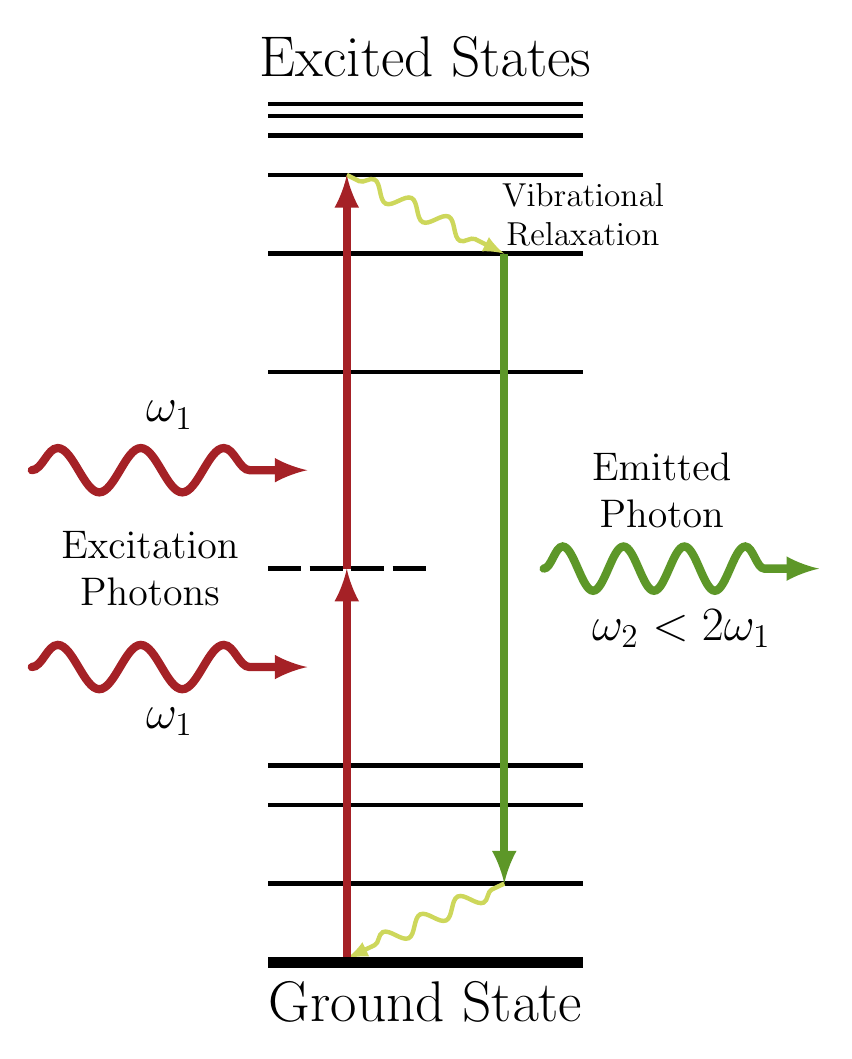
\begin{tikzpicture}

\draw [ultra thick] (4,12.90) -- (8,12.90);
\draw [ultra thick] (4,12.75) -- (8,12.75);
\draw [ultra thick] (4,12.50) -- (8,12.50);
\draw [ultra thick] (4,12.00) -- (8,12.00);
\draw [ultra thick] (4,11.00) -- (8,11.00);
\draw [ultra thick] (4,09.50) -- (8,09.50);

\draw [ultra thick,dash pattern=on 12pt off 3pt] (4,7) -- (6,7);

\draw [ultra thick] (4,4.50) -- (8,4.50);
\draw [ultra thick] (4,4.00) -- (8,4.00);
\draw [ultra thick] (4,3.00) -- (8,3.00);

\draw [-latex,decorate,
    decoration={snake,amplitude=3,segment length=15,pre length=5,post length=5},
    ultra thick,yellowgreen] (5,12) -- (7,11);
\draw [-latex,line width=3pt,green] (7,11) -- (7,3);
\draw [-latex,decorate,
    decoration={snake,amplitude=3,segment length=15,pre length=5,post length=5},
    ultra thick,yellowgreen] (7,3) -- (5,2.05);

\draw [-latex,line width=3pt,darkred] (5,7) -- (5,12);
\draw [-latex,line width=3pt,darkred] (5,2) -- (5,7);

\draw [line width=4pt] (4,2) -- (8,2);

% light beams yo
\draw [-latex,decorate,
       decoration={snake,amplitude=8,segment length=30,post length=10},
       line width=3pt,darkred,line cap = round] (1,8.25) -- (4.5,8.25)
       node [black,midway,above=10] {{\LARGE $\omega_{1}$}};
\draw [-latex,decorate,
       decoration={snake,amplitude=8,segment length=30,post length=10},
       line width=3pt,darkred,line cap = round] (1,5.75) -- (4.5,5.75)
       node [black,midway,below=10] {{\LARGE $\omega_{1}$}};
\draw [-latex,decorate,
       decoration={snake,amplitude=8,segment length=22, post length=10},
       line width=3pt,green,line cap = round] (7.5,7) -- (11,7)
       node [black,midway,below=10]
       {{\LARGE $\omega_{2}  <2\omega_{1}$}};

% some text
\node at (6,13.5) {\huge Excited States};
\node at (6,01.5) {\huge Ground State};
\node [align=center] at (2.5,7.0) {\Large Excitation\\[5pt]\Large Photons};
\node [align=center] at (9,8.0) {\Large Emitted\\[5pt]\Large Photon};
\node [align=center] at (8,11.5) {\large Vibrational\\[2pt]\large Relaxation};
% \node at (4.2,0.7) {\Huge Centrosymmetric Bulk};

\end{tikzpicture}

\end{document}
